\chapter{Fourier, Bandwidth, and Coherence Time}
\label{chap:e02}

\begin{chapteropening}
In the previous chapter we regarded light as ``a rapidly rotating complex-amplitude arrow,'' and also conceded that the detector is too slow and can only record the intensity after it has been smoothed. But ``too slow'' relative to what, exactly? And how long can the phase of the light stay ordered before it scrambles? To answer these questions, we must first learn a universal language: any stretch of a wave, no matter how complicated, can be decomposed into a heap of pure single-frequency sinusoids, just as a chord can always be broken down into individual pure tones. This chapter first makes this ``tone-decomposition'' language (Fourier analysis) clear, then uses it to derive three quantities we will use again and again later: the bandwidth \(\Delta\nu\), the coherence time \(\tau_c\), and the autocorrelation and power spectrum that link the two. By the end you will understand why a nanosecond-scale time gate in fact packs hundreds or thousands of ``coherence times'' into it.
\end{chapteropening}

\section{Any Wave Is a Superposition of Pure Tones}
\label{sec:e02-fourier-idea}

Let us first build the picture. Imagine you hold a signal \(f(t)\) that varies with time: it could be the displacement of a violin string, or the electric field at some point on the detection surface. Fourier's insight is this: this signal is never ``one solid block,'' but the result of many sinusoids of different frequencies superposed together. The low-frequency sinusoids sketch out the broad outline, the high-frequency sinusoids fill in the sharp detail; add them up according to their respective ``weights'' and the original signal is recovered. This list of ``how much weight each frequency carries'' is called the \textbf{spectrum} of the signal.

First consider the most easily imagined case: the signal is periodic with period \(T\), that is, \(f(t+T)=f(t)\). In this case the allowed frequencies are not continuous but come rung by rung as harmonics: the fundamental frequency \(\nu_1=1/T\) and its integer multiples \(\nu_n=n/T\). The Fourier series says that such a periodic signal can be written as
\begin{equation}
  f(t)=\sum_{n=-\infty}^{+\infty} c_n\,e^{\,i\,2\pi\nu_n t},
  \qquad
  \nu_n=\frac{n}{T},
  \label{eq:e02-fourier-series}
\end{equation}
\begin{formulaexplain}
\(f(t)\) is the signal of period \(T\); \(\nu_n=n/T\) is the frequency of the \(n\)-th harmonic; the complex coefficient \(c_n\) is the ``weight'' this harmonic carries in the signal (containing both amplitude and phase). The whole equation says: a periodic signal is a sum of a stack of discrete pure tones.
\end{formulaexplain}
Here each term \(e^{i2\pi\nu_n t}\) is a ``unit arrow rotating uniformly at frequency \(\nu_n\),'' and the complex coefficient \(c_n\) sets how long the arrow is (amplitude) and where it initially points (phase). Since \(e^{i2\pi\nu_n t}\) is a dimensionless pure-phase factor, the dimension of the signal \(f(t)\) is carried entirely by the complex coefficients \(c_n\); the unit of \(\nu_n\) is the hertz (\({\rm Hz}={\rm s^{-1}}\)). To extract the weight of a particular harmonic, one need only ``beat time'' between the signal and that harmonic: integrate over one period, and orthogonality makes all the other harmonics cancel, leaving only the one term we want:
\[
  c_n=\frac{1}{T}\int_{0}^{T} f(t)\,e^{-\,i\,2\pi\nu_n t}\,dt .
\]
The key fact used here is that different harmonics are mutually orthogonal: \(\frac{1}{T}\int_0^T e^{i2\pi(m-n)t/T}\,dt=\delta_{mn}\) (when \(m=n\) the integrand is identically 1 and the integral gives 1; when \(m\neq n\) it is a complex exponential over one full period, whose positives and negatives cancel to give 0). This is the first ``known result'' we call upon by name, and we will use it again and again later.

Now imagine the period \(T\) growing longer and longer. The spacing of the harmonics \(\Delta\nu=\nu_{n+1}-\nu_n=1/T\) becomes denser and denser; when \(T\to\infty\), the signal is no longer periodic, and the rung-by-rung discrete frequencies merge into a continuous frequency axis. The step most easily skipped here is: where exactly did that normalization factor \(1/T\) in the series go? Making it clear requires only a small trick: in the synthesis formula \eqref{eq:e02-fourier-series}, attach to each term a ``frequency-spacing'' factor \(\Delta\nu\) (recall \(\Delta\nu=1/T\)), multiplying by one and dividing by one, leaving the equation unchanged:
\[
  f(t)=\sum_{n} c_n\,e^{\,i2\pi\nu_n t}
      =\sum_{n} \frac{c_n}{\Delta\nu}\,e^{\,i2\pi\nu_n t}\,\Delta\nu .
\]
This step changes nothing; it merely arranges the whole sum into the standard shape of a Riemann sum \(\sum_n g(\nu_n)\,\Delta\nu\): each term carrying the small slice of frequency width \(\Delta\nu\) it occupies. When \(T\to\infty\), \(\Delta\nu\to d\nu\), the Riemann sum converges to an integral, the discrete frequency \(\nu_n\) becomes a continuous variable \(\nu\), and the combination \(c_n/\Delta\nu\) in the parentheses converges to a continuous \textbf{spectral density}
\[
  \tilde f(\nu)\;=\;\frac{c_n}{\Delta\nu}\;=\;c_n\,T .
\]
So the fate of the \(1/T\) is settled: it did not vanish into thin air, but was absorbed by \(\Delta\nu=1/T\) into the integration measure \(d\nu\), at the cost that the spectral density \(\tilde f(\nu)\) is larger than the original series coefficient \(c_n\) by a full factor of \(T\) (this also lines up with the analysis formula: multiply both sides of \(c_n=\frac1T\int_0^T f\,e^{-i2\pi\nu_n t}dt\) by \(T\), the \(1/T\) on the right cancels exactly, and what remains is \(\tilde f(\nu)=\int f\,e^{-i2\pi\nu t}dt\)). In this way the sum \(\sum_n\) cleanly becomes the integral \(\int d\nu\), and we have passed from the Fourier series to the Fourier transform. We shall not fuss over the remaining mathematical details of convergence, keeping only this physical intuition: the spectrum of a non-periodic signal is continuous, every frequency may appear, each carrying its own weight. The Fourier transform pair is written
\begin{equation}
  \tilde f(\nu)=\int_{-\infty}^{+\infty} f(t)\,e^{-\,i\,2\pi\nu t}\,dt,
  \qquad
  f(t)=\int_{-\infty}^{+\infty} \tilde f(\nu)\,e^{+\,i\,2\pi\nu t}\,d\nu .
  \label{eq:e02-fourier-transform}
\end{equation}
\begin{formulaexplain}
The left equation ``decomposes'' the time signal \(f(t)\) into the spectrum \(\tilde f(\nu)\); the right equation ``recomposes'' the spectrum back into the signal. \(e^{\mp i2\pi\nu t}\) is a pure tone of frequency \(\nu\). Decomposition and recomposition are inverses of each other, with no gain or loss of information.
\end{formulaexplain}
The two equations are inverses of each other: the left (the analysis equation) is like using a row of tuned tuning forks to ``listen'' for how strong each frequency in the signal is, while the right (the synthesis equation) is like replaying those pure tones according to their weights and reassembling the original signal. Note that \(\tilde f(\nu)\) is generally complex: its modulus \(|\tilde f(\nu)|\) says how much weight this frequency carries, and its argument gives the phase of this frequency component. If the frequency axis is replaced by the wavelength axis, this is exactly the abstract version of the spectral-line curve a spectrograph spits out. When later in the book we speak of ``spectral-line width,'' ``filter bandwidth,'' and ``coherence function,'' the underlying machinery is always this pair of equations.

To sum up in one sentence: the Fourier transform is a ``decompose-and-recompose'' machine that translates ``varies with time'' into ``composed of which frequencies.'' Next we set it to its first genuinely useful task.

\section{The Finite-Length Wave Packet: The Shorter in Time, the Broader in Frequency}
\label{sec:e02-wavepacket}

Real light is never an infinitely long, perfectly single-frequency sinusoid. Each time an atom in a star emits, it radiates only an extremely short wave train before being interrupted by a collision; a filter, too, passes only a small band of frequencies. So what we always face is a \textbf{wave packet}: a stretch of oscillation with a beginning and an end, whose frequency is not perfectly single either. Hidden here is an iron law that runs through the whole book: \emph{the shorter a wave is in time, the broader it is in frequency}; conversely, to be extremely pure in frequency, the wave train must be extremely long.

Why? The intuition is this: an infinitely long perfect sinusoid needs only one frequency to describe, and its spectrum is a single needle. But once you ``cut it short'' (multiply it by an envelope of finite width), you have forcibly snuffed it out at both ends, and the very act of ``snuffing out'' requires additional frequency components to accomplish (just as sounding an extremely brief ``tap'' must call upon a very wide band of pitches). The shorter the wave train, the more abruptly it is snuffed, and the wider the frequencies needed. Written as an order-of-magnitude relation, this is the famous
\begin{equation}
  \Delta\nu\,\Delta t \;\gtrsim\; 1 ,
  \label{eq:e02-bandwidth-time}
\end{equation}
\begin{formulaexplain}
\(\Delta t\) is the temporal duration width of the wave packet, and \(\Delta\nu\) is its spread in frequency. Their product cannot be smaller than about 1: the narrower in time, the necessarily broader in frequency. This is a universal constraint of the Fourier transform, not an instrumental defect.
\end{formulaexplain}
In the formula the unit of \(\Delta t\) is the second and the unit of \(\Delta\nu\) is the hertz, so the product is dimensionless. Note that this is not the Heisenberg uncertainty principle but a purely classical wave property; the quantum-mechanical \(\Delta E\,\Delta t\gtrsim\hbar\) is merely its counterpart after multiplying by \(E=h\nu\). The ``\(\gtrsim\)'' in Eq.~\eqref{eq:e02-bandwidth-time} reminds us that it is an order-of-magnitude relation, with the precise coefficient depending on how ``width'' and the envelope shape are defined. Below we use an example that can be computed to the end to turn this inequality into an equality.

\paragraph{Explicit calculation for a Gaussian wave packet}

Take an oscillation modulated by a Gaussian envelope; writing it in complex form is the least laborious:
\[
  f(t)=e^{-\,t^{2}/(2\sigma_t^{2})}\;e^{\,i\,2\pi\nu_0 t}.
\]
Here \(\nu_0\) is the carrier frequency (about \(6\times10^{14}\,{\rm Hz}\) for visible light), and \(\sigma_t\) is the temporal width of the envelope (in seconds): \(|f|\) reaches its peak at \(t=0\) and decays to \(e^{-1/2}\) of the peak at \(|t|\sim\sigma_t\). Let us find its spectrum \(\tilde f(\nu)\). Substituting into the definition \eqref{eq:e02-fourier-transform}:
\[
  \tilde f(\nu)=\int_{-\infty}^{+\infty}
  e^{-\,t^{2}/(2\sigma_t^{2})}\,e^{\,i\,2\pi\nu_0 t}\,e^{-\,i\,2\pi\nu t}\,dt
  =\int_{-\infty}^{+\infty}
  e^{-\,t^{2}/(2\sigma_t^{2})}\,e^{-\,i\,2\pi(\nu-\nu_0)t}\,dt .
\]
Combining the exponents into the standard form of ``quadratic $+$ linear term,'' let \(a=\dfrac{1}{2\sigma_t^{2}}\) and \(b=i\,2\pi(\nu-\nu_0)\); the integrand is \(e^{-a t^{2}-b t}\). Here we call upon a known result by name, the completing-the-square formula for the \textbf{Gaussian integral}:
\[
  \int_{-\infty}^{+\infty} e^{-a t^{2}-b t}\,dt
  =\sqrt{\frac{\pi}{a}}\;e^{\,b^{2}/(4a)},
  \qquad(a>0).
\]
(Its provenance is to complete the exponent into \(-a(t+\tfrac{b}{2a})^2+\tfrac{b^2}{4a}\), then use the most basic \(\int e^{-a u^2}du=\sqrt{\pi/a}\).) Substituting \(a,b\):
\[
  \sqrt{\frac{\pi}{a}}=\sqrt{2\pi}\,\sigma_t,
  \qquad
  \frac{b^{2}}{4a}
  =\frac{\bigl[i\,2\pi(\nu-\nu_0)\bigr]^{2}}{4/(2\sigma_t^{2})}
  =\frac{-4\pi^{2}(\nu-\nu_0)^{2}}{2/\sigma_t^{2}}
  =-2\pi^{2}\sigma_t^{2}(\nu-\nu_0)^{2}.
\]
So the spectrum is
\begin{equation}
  \tilde f(\nu)=\sqrt{2\pi}\,\sigma_t\;
  e^{-\,2\pi^{2}\sigma_t^{2}(\nu-\nu_0)^{2}}.
  \label{eq:e02-gaussian-spectrum}
\end{equation}
\begin{formulaexplain}
The spectrum of a Gaussian wave packet is still a Gaussian, centred on the carrier frequency \(\nu_0\). In the exponent, the larger \(\sigma_t\) (the longer the wave train), the narrower the frequency Gaussian. The widths of the time and frequency Gaussians are inversely proportional.
\end{formulaexplain}
This is a beautiful self-consistent result: \emph{the Fourier transform of a Gaussian is still a Gaussian}. Writing the exponent of Eq.~\eqref{eq:e02-gaussian-spectrum} in the standard Gaussian form \(e^{-(\nu-\nu_0)^2/(2\sigma_\nu^2)}\), we read off the frequency width:
\[
  \frac{1}{2\sigma_\nu^{2}}=2\pi^{2}\sigma_t^{2}
  \quad\Longrightarrow\quad
  \sigma_\nu=\frac{1}{2\pi\,\sigma_t}.
\]
The time width \(\sigma_t\) and the frequency width \(\sigma_\nu\) are indeed inversely proportional. Multiplying them together, the carrier, amplitude, and all such details cancel out, leaving only a pure number:
\begin{equation}
  \sigma_t\,\sigma_\nu=\frac{1}{2\pi}\approx0.16 .
  \label{eq:e02-gaussian-product}
\end{equation}
\begin{formulaexplain}
The Gaussian wave packet makes the product of time width and frequency width attain its minimum value \(1/2\pi\). Any other shape of wave packet only makes it larger. This is the precise lower-bound version of the ``\(\gtrsim 1\)'' in Eq.~\eqref{eq:e02-bandwidth-time}.
\end{formulaexplain}
Here we must beware of a numerical ``tension'': \(1/2\pi\approx0.16\) and the ``\(\gtrsim1\)'' in Eq.~\eqref{eq:e02-bandwidth-time} look like they differ by about a factor of 6, and the reader will inevitably ask ``how can the lower bound be 0.16 rather than 1?'' The answer lies entirely in the calibre of the word ``width.'' The \(\sigma_t,\sigma_\nu\) in Eq.~\eqref{eq:e02-gaussian-product} are the \emph{standard deviations} of the amplitude Gaussian, whereas the ``width'' often spoken of experimentally usually means the \emph{full width at half maximum} (FWHM) \(\Delta\). For a Gaussian the conversion between the two is \(\Delta=2\sqrt{2\ln2}\,\sigma\approx2.35\,\sigma\), so
\[
  \Delta\nu\,\Delta t=(2.35)^2\,\sigma_\nu\sigma_t
  \approx\frac{2.35^2}{2\pi}\approx0.88\sim1 .
\]
Once the full width at half maximum is used as the measure, the product immediately returns to order 1, in complete agreement with Eq.~\eqref{eq:e02-bandwidth-time}. So \(1/2\pi\) and 1 do not contradict each other; they differ only by a numerical coefficient determined by ``whether you define the width as the standard deviation or the full width at half maximum'': the physics is one and the same, while the number floats with the calibre. Understanding this, one can confidently put the order-of-magnitude inequality \eqref{eq:e02-bandwidth-time} into practice: the Gaussian wave packet is the extreme case of ``simultaneously most compact in time and frequency,'' attaining the lower bound; replace it with a square-wave envelope, a Lorentzian line shape, or a wave train randomly interrupted by collisions, and the product only grows larger, but always of order 1. So no matter how the light is produced, as long as it lasts a time \(\Delta t\), its frequency spreads out at least about \(1/\Delta t\) wide. Remember this one point, and in the next section we can compute the ``bandwidth'' and the ``coherence time'' in one breath. Figure~\ref{fig:e02-wave-packet} draws this iron law as a clear-at-a-glance comparison.

\begin{figure}[tbp]
\centering
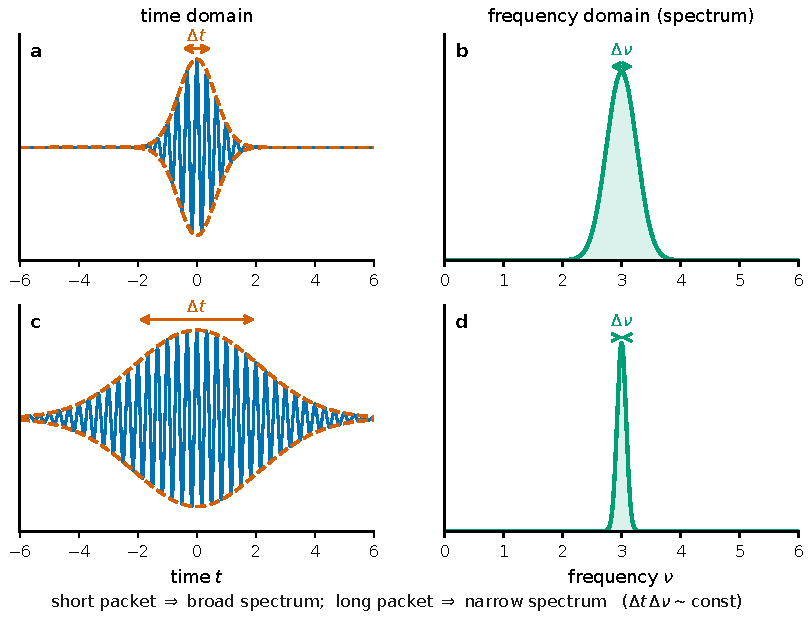
\includegraphics[width=0.9\linewidth]{figures/generated/edu_ch02/e02_wave_packet_spectrum.pdf}
\caption{The ``time--frequency reciprocity'' of finite-length wave packets. The top row is a short wave packet: pinched very narrow in time (\(\Delta t\) small, orange double arrow), yet its spectrum spreads very wide (\(\Delta\nu\) large); the bottom row is a long wave packet: stretched very long in time, its spectrum instead squeezed into a narrow peak. The orange dashed line is the envelope, the green is the corresponding spectrum. The product \(\Delta t\,\Delta\nu\) of both rows is about the same constant: this is precisely the picture of Eq.~\eqref{eq:e02-bandwidth-time}.}
\label{fig:e02-wave-packet}
\end{figure}

\section{Computing the Bandwidth as a Real Number}
\label{sec:e02-bandwidth}

In astronomical observation we usually do not know the frequency bandwidth \(\Delta\nu\) directly, but rather the filter's central wavelength \(\lambda\) and wavelength bandwidth \(\Delta\lambda\) (for example, ``500 nanometres centre, 1 nanometre half-width''). To translate it into a frequency bandwidth, we need only differentiate the relation between \(\nu\) and \(\lambda\) once. Frequency and wavelength are linked by the speed of light:
\[
  \nu=\frac{c}{\lambda}.
\]
Here \(c\approx3\times10^{10}\,{\rm cm\,s^{-1}}\) is the speed of light; following the book's CGS convention throughout, the wavelength \(\lambda\) is measured in centimetres and the frequency \(\nu\) in hertz. Differentiating with respect to \(\lambda\) (this step cannot be skipped), using \(\dfrac{d}{d\lambda}\bigl(c\lambda^{-1}\bigr)=-c\lambda^{-2}\):
\[
  \frac{d\nu}{d\lambda}=-\frac{c}{\lambda^{2}}.
\]
The negative sign indicates that frequency decreases as wavelength increases, which is the expected inverse relation; what we care about is the magnitude of the bandwidth, so we take the absolute value and replace the differential \(d\lambda\) with a finite small bandwidth \(\Delta\lambda\) (as long as \(\Delta\lambda\ll\lambda\), approximating the finite difference by the differential is accurate enough):
\begin{equation}
  \Delta\nu\;\simeq\;\frac{c\,\Delta\lambda}{\lambda^{2}} .
  \label{eq:e02-bandwidth-conversion}
\end{equation}
\begin{formulaexplain}
\(\Delta\nu\) is the frequency bandwidth, \(\Delta\lambda\) is the wavelength bandwidth, \(\lambda\) is the central wavelength, and \(c\) is the speed of light. For the same \(\Delta\lambda\), the shorter the wavelength (the smaller \(\lambda^2\)), the larger the frequency bandwidth converted.
\end{formulaexplain}
Note that the denominator is \(\lambda^{2}\) rather than \(\lambda\): this reminds us that the same ``1 nanometre'' wavelength window corresponds to a larger frequency bandwidth at the blue end than at the red end. Now let us put in real numbers. Take a visible-light filter, \(\lambda=500\,{\rm nm}=5\times10^{-5}\,{\rm cm}\), \(\Delta\lambda=1\,{\rm nm}=1\times10^{-7}\,{\rm cm}\):
\[
  \Delta\nu\simeq
  \frac{(3\times10^{10}\,{\rm cm\,s^{-1}})\times(1\times10^{-7}\,{\rm cm})}
       {(5\times10^{-5}\,{\rm cm})^{2}}
  =\frac{3\times10^{3}}{2.5\times10^{-9}}\,{\rm Hz}
  =1.2\times10^{12}\,{\rm Hz}.
\]
That is, about \(1.2\,{\rm THz}\) (terahertz). Please fix this order of magnitude firmly in mind: a 1-nanometre filter that looks ``very narrow'' in fact passes a window a trillion-plus hertz wide in frequency. Compared with the carrier frequency \(\nu_0\sim6\times10^{14}\,{\rm Hz}\), this window occupies only \(0.2\%\), and in the spectroscopic sense is indeed ``narrow''; but once converted to a timescale, it will bring about an astonishing shortness. This is precisely the protagonist of the next section.

\section{Coherence Time: How Long the Wave Remembers Its Own Phase}
\label{sec:e02-coherence-time}

Now let us translate the bandwidth of the previous section into time. Return to the iron law \eqref{eq:e02-bandwidth-time}: a stretch of light whose frequency spreads out \(\Delta\nu\) can at most keep ``coordinated'' in time for about \(\Delta t\sim1/\Delta\nu\). Let us give this time a name, the \textbf{coherence time} \(\tau_c\):
\begin{equation}
  \tau_c\;\simeq\;\frac{1}{\Delta\nu}
  \;\simeq\;\frac{\lambda^{2}}{c\,\Delta\lambda} .
  \label{eq:e02-coherence-time}
\end{equation}
\begin{formulaexplain}
\(\tau_c\) is the coherence time, in seconds; the wider the bandwidth \(\Delta\nu\), the shorter the coherence time. The second equality is just Eq.~\eqref{eq:e02-bandwidth-conversion} substituted in, expressing it in wavelength terms. It is the length of time light ``remembers its own phase,'' not the time resolution of the detector.
\end{formulaexplain}
How should we understand \(\tau_c\)? Think of light as that rotating complex-amplitude arrow. If the light were ideally single-frequency, the arrow would turn uniformly at constant angular velocity, and by glancing at where it points this instant you could accurately predict where it will point a microsecond later, or an hour later: it ``remembers its phase forever.'' But real light has bandwidth: it mixes in a whole crowd of arrows with slightly different frequencies, turning at slightly different rates; at first orderly, they spread apart as they turn, and the phase of the resultant arrow becomes ever less predictable. \(\tau_c\) is the time needed ``to go from orderly to scattered'': past \(\tau_c\), the light has basically forgotten its phase from \(\tau_c\) ago. The wider the bandwidth, the greater the spread of rates mixed in, and the faster it forgets.

Substituting the number from the previous section, \(\Delta\nu\simeq1.2\times10^{12}\,{\rm Hz}\):
\[
  \tau_c\simeq\frac{1}{1.2\times10^{12}\,{\rm Hz}}
  \approx8.3\times10^{-13}\,{\rm s}
  \approx0.8\,{\rm ps}.
\]
Less than one picosecond (\(1\,{\rm ps}=10^{-12}\,{\rm s}\)). This is the coherence time given by that ``very narrow'' 1-nanometre filter: the light can remember its own phase for only about 0.8 picoseconds, then it turns the page.

The reason this number took a whole chapter to prepare is that there is a jaw-dropping gulf between it and the capability of the detector. The fastest single-photon detectors (avalanche photodiode APD, photomultiplier tube PMT) have a time response of roughly 100 picoseconds to 1 nanosecond. Comparing with the coherence time:
\[
  \frac{\Delta t_{\rm det}}{\tau_c}\sim
  \frac{100\,{\rm ps}\;\text{to}\;1\,{\rm ns}}{0.8\,{\rm ps}}
  \approx1.2\times10^{2}\;\text{to}\;1.2\times10^{3}.
\]
That is, the width of one time gate (time bin) of the detector is \emph{hundreds to thousands of times} the coherence time. In other words, every time you record the intensity of one time gate, you are in fact averaging together hundreds or thousands of mutually incoherent, independent wave trains. The detector has no time to see clearly the phase fluctuation of any single wave train; what it sees is always the average energy after hundreds or thousands of coherence times have been smoothed out. This conclusion (``one time gate averages \(N\sim10^{2}\)--\(10^{3}\) coherence times'') will recur again and again later when we discuss photon statistics, bunching, and intensity interferometry, and directly determines by how many times the signal we can measure is diluted.

\begin{figure}[tbp]
\centering
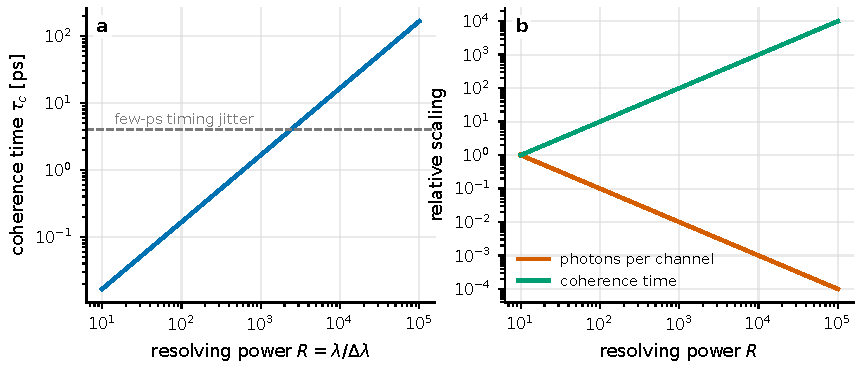
\includegraphics[width=0.85\linewidth]{figures/generated/chapter_06/ch06_spectral_resolution_coherence.pdf}
\caption{Spectral resolution and coherence time are two faces of the same thing. The narrower the spectral line (bandwidth \(\Delta\nu\)), the longer the corresponding coherence time \(\tau_c\simeq1/\Delta\nu\); conversely broadband light has an extremely short coherence time. The figure places the ps-scale \(\tau_c\) given by a visible-light broadband filter alongside the detector's 100\,ps--1\,ns response, showing that one time gate contains a great many mutually incoherent wave trains.}
\label{fig:e02-spectral-coherence}
\end{figure}

A one-sentence summary: bandwidth and coherence time are two faces of the same coin, \(\tau_c\simeq1/\Delta\nu\). Under visible-light broadband, \(\tau_c\) is as short as a picosecond, while the detector is as slow as more than a hundred picoseconds, the two differing by more than a hundredfold: this gulf is the backdrop for all the intensity measurements that follow.

\section{Autocorrelation and Power Spectrum: Toward the Coherence Function}
\label{sec:e02-autocorrelation}

Earlier we described the coherence time as ``\(\tau_c\) is the length of the phase memory,'' which is a qualitative statement. How do we quantify ``memory'' into a computable, measurable curve? The answer is the \textbf{autocorrelation function}. Its idea is extremely plain: multiply the signal by ``itself delayed by \(\tau\),'' then average, and see how alike they still are. For a (stationary) signal \(f(t)\), define
\begin{equation}
  \Gamma(\tau)=\bigl\langle f^{*}(t)\,f(t+\tau)\bigr\rangle
  =\lim_{T\to\infty}\frac{1}{T}\int_{0}^{T} f^{*}(t)\,f(t+\tau)\,dt ,
  \label{eq:e02-autocorrelation}
\end{equation}
\begin{formulaexplain}
\(\Gamma(\tau)\) is the autocorrelation function; \(\tau\) is the time delay; the angle brackets (or time integral) denote the time average; \(f^*\) is the complex conjugate. It measures the similarity between ``the signal now'' and ``the signal after \(\tau\).''
\end{formulaexplain}
When the delay \(\tau=0\), \(\Gamma(0)=\langle|f|^{2}\rangle\) is the average intensity of the signal (a positive real number, the maximum value). As \(\tau\) increases, if the signal still ``remembers'' itself, the phases of \(f^*(t)\) and \(f(t+\tau)\) remain in step, the product does not cancel after averaging, and \(\Gamma\) stays large; once \(\tau\) exceeds the coherence time, the two phases have long gone their separate ways, randomly distributed, the positive and negative products cancel in the average, and \(\Gamma\to0\). So \emph{the width over which the autocorrelation function decays from its peak to zero is precisely the coherence time \(\tau_c\)}. This turns the vague ``memory length'' of the previous section into the width of a curve, computable and measurable. The left panel of Figure~\ref{fig:e02-coherence} shows exactly this decay: the wider the bandwidth, the faster the normalized autocorrelation drops and the shorter the coherence time; the right panel draws the scaling \(\tau_c\simeq1/\Delta\nu\) as a straight line.

\begin{figure}[tbp]
\centering
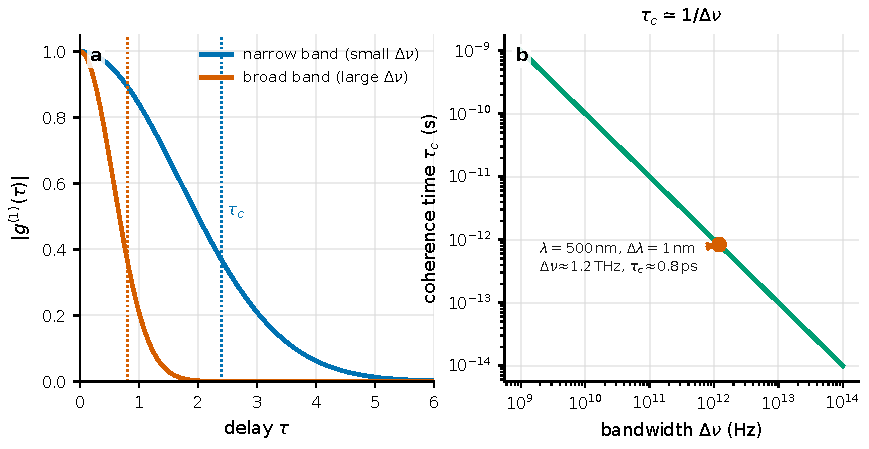
\includegraphics[width=0.92\linewidth]{figures/generated/edu_ch02/e02_coherence_bandwidth.pdf}
\caption{Coherence time and bandwidth are reciprocals of each other. Left: the normalized autocorrelation (which is also the first-order coherence \(|g^{(1)}(\tau)|\) to be formally defined later) decays with the delay \(\tau\); the wider the bandwidth (orange), the faster it drops and the shorter the coherence time \(\tau_c\), while the narrower the bandwidth (blue) the longer it ``remembers.'' Right: \(\tau_c\simeq1/\Delta\nu\) is a straight line in log-log coordinates, with the orange dot marking the \(\Delta\nu\approx1.2\,{\rm THz}\), \(\tau_c\approx0.8\,{\rm ps}\) given by the \(500\,{\rm nm}\), \(1\,{\rm nm}\) filter.}
\label{fig:e02-coherence}
\end{figure}

Finally we point out a beautiful and profound theorem that ties the chapter's two main threads (spectrum and coherence) into a single knot. This is the \textbf{Wiener--Khinchin theorem}: the \textbf{power spectrum} \(S(\nu)\) of a signal is exactly the Fourier transform of its autocorrelation function:
\begin{equation}
  S(\nu)=\int_{-\infty}^{+\infty}\Gamma(\tau)\,e^{-\,i\,2\pi\nu\tau}\,d\tau .
  \label{eq:e02-wiener-khinchin}
\end{equation}
\begin{formulaexplain}
\(S(\nu)\) is the power spectrum, telling you how much power each frequency carries; \(\Gamma(\tau)\) is the autocorrelation function. The two are a Fourier-transform pair. ``Which frequencies the signal contains'' and ``how long the signal remembers itself'' are two ways of saying the same thing.
\end{formulaexplain}
The meaning of this theorem is worth savouring slowly. It says: \emph{you need not actually measure the spectrum; just measure the autocorrelation function, take one Fourier transform, and you get the power spectrum; and vice versa}. This is exactly the rigorous embodiment of Eq.~\eqref{eq:e02-bandwidth-time}: the width of the autocorrelation (the coherence time \(\tau_c\)) and the width of the power spectrum (the bandwidth \(\Delta\nu\)) are a Fourier pair, one narrow means the other must be broad, with a product of about 1. Looking back at the Gaussian wave packet section: the time Gaussian and the frequency Gaussian are Fourier transforms of each other with inversely proportional widths, which is precisely one concrete sample of the Wiener--Khinchin theorem.

Why, in an astronomy book, do we introduce the autocorrelation so solemnly? Because the structure of that \(\langle f^*(t)f(t+\tau)\rangle\) in Eq.~\eqref{eq:e02-autocorrelation} is, almost unchanged, exactly the \textbf{first-order coherence function} \(g^{(1)}(\tau)\) to be defined later: just replace \(f\) with the electric field and normalize. That is, the autocorrelation function of this chapter is the ``classical rehearsal'' of the coherence function. When we formally introduce \(g^{(1)}\) and \(g^{(2)}\) after Chapter~\ref{chap:e05}, you will find they are not mysterious at all: \(g^{(1)}\) measures the autocorrelation of the electric field (phase memory), and its width is the \(\tau_c\) here; and between the spectral-line shape of a star and it, the bridge is precisely the Wiener--Khinchin theorem. The language this chapter has built (spectrum, bandwidth, coherence time, autocorrelation) is the foundation of the whole theory of coherence.

\section{Chapter Summary}
\label{sec:e02-summary}

\begin{itemize}
  \item \textbf{The Fourier idea}: any wave is a superposition of pure tones. A periodic signal gives discrete harmonics (Fourier series), a non-periodic signal gives a continuous spectrum (Fourier transform, Eq.~\eqref{eq:e02-fourier-transform}). The spectrum is the list of ``how much weight each frequency carries.''
  \item \textbf{Time--frequency reciprocity}: the shorter the wave train, the broader the frequency, \(\Delta\nu\,\Delta t\gtrsim1\) (Eq.~\eqref{eq:e02-bandwidth-time}). The Gaussian wave packet attains the most compact lower bound \(\sigma_t\sigma_\nu=1/2\pi\), and its Fourier transform is still a Gaussian.
  \item \textbf{Bandwidth conversion}: differentiating \(\nu=c/\lambda\) gives \(\Delta\nu\simeq c\,\Delta\lambda/\lambda^{2}\). A 500\,nm, 1\,nm filter gives \(\Delta\nu\approx1.2\times10^{12}\,{\rm Hz}\).
  \item \textbf{Coherence time}: \(\tau_c\simeq1/\Delta\nu\approx0.8\,{\rm ps}\). It is the length of time light remembers its own phase. The detector's 100\,ps--1\,ns response is a hundred to a thousand times longer: one time gate averages hundreds to thousands of coherence times.
  \item \textbf{Autocorrelation and power spectrum}: the decay width of the autocorrelation \(\Gamma(\tau)\) is the \(\tau_c\); the Wiener--Khinchin theorem (Eq.~\eqref{eq:e02-wiener-khinchin}) says the power spectrum is the Fourier transform of the autocorrelation. This is precisely the forerunner of the first-order coherence function \(g^{(1)}\).
\end{itemize}

\noindent\textbf{Questions to Ponder}:
\begin{enumerate}
  \item If the filter is changed to a \(10\,{\rm nm}\) bandwidth, what does the coherence time become? And how many coherence times are averaged in one \(1\,{\rm ns}\) time gate of the detector?
  \item A wave train interrupted by collisions on average once every \(\tau_c\), roughly how wide is its spectral line? (Hint: work backward from Eq.~\eqref{eq:e02-bandwidth-time}.)
  \item Why is ``measuring the autocorrelation function'' equivalent in information to ``measuring the spectrum''? What role does the Wiener--Khinchin theorem play in this?
\end{enumerate}
